\documentclass{article}
\pdfminorversion=4
%
%	PAGE GEOMETRY
%
\usepackage{geometry}
\geometry{
	paperwidth=15cm, %7cm, %7cm, % 15cm
	paperheight=4cm,
	layouthoffset=0cm,
	layoutvoffset=0cm,
	hmargin={0cm,0cm},
	vmargin={0cm,0cm}
}
%

%
%	FILE ENCODING
%
\usepackage[utf8]{inputenc}
%

%
%	AMS STUFF
%
\usepackage{amsfonts}
\usepackage{amsthm}
\newtheorem{theorem}{Theorem}
%

%
%	ACRONYMS
%
\usepackage{acronym}
\acrodef{GA}{Genetic algorithms}
\acrodef{rmse}[error]{root-mean-square error}
\acrodef{GAPoly}[{\sc GAPoly}]{Genetic Algorithms for Polynomials}
%

%
%	FIGURE AND STUFF ENVIRONMENT
%
\usepackage{graphicx}
%

%
%	TIKZ AND RELATED STUFF
%
\usepackage{pgfplots}
\pgfplotsset{compat=newest}
\usepgfplotslibrary{statistics}
\usetikzlibrary{external}
\tikzexternalize[prefix=tikz/]
%
%
%%%%%%%%%%%%%%%%%%%%%%%%%%%%%%%%%%%%%%%%%%%%%%%%%%%%%%%%%%%%%%%%%%%%%%%%%
%
%	EMBEDDED DATASETS
%
\begin{filecontents}{inlambdas.dat}
2.474 2.460
2.414 2.392
2.414 2.392
2.414 2.392
2.407 2.392
2.407 2.392
2.317 2.331
2.351 2.331
2.330 2.331
2.314 2.318
2.251 2.318
2.251 2.318
2.251 2.318
2.275 2.318
2.275 2.318
2.275 2.318
2.275 2.318
2.275 2.296
2.275 2.296
2.268 2.296
2.268 2.296
2.268 2.296
2.225 2.296
2.225 2.296
2.225 2.296
2.225 2.296
2.225 2.296
2.225 2.296
2.225 2.268
2.225 2.268
2.225 2.268
2.225 2.261
2.225 2.261
2.225 2.261
2.225 2.261
2.225 2.261
2.225 2.261
2.225 2.261
2.225 2.261
2.225 2.261
2.225 2.261
2.225 2.261
2.225 2.261
2.225 2.261
2.225 2.261
2.225 2.261
2.225 2.261
2.225 2.261
2.225 2.261
2.225 2.261
2.225 2.261
2.225 2.261
2.225 2.261
2.225 2.261
2.225 2.261
2.225 2.261
2.225 2.261
2.225 2.261
2.225 2.261
2.225 2.247
2.225 2.247
2.200 2.247
2.200 2.247
2.200 2.247
2.200 2.247
2.200 2.247
2.200 2.247
2.200 2.247
2.200 2.247
2.200 2.247
2.200 2.247
2.200 2.247
2.200 2.247
2.200 2.247
2.200 2.247
2.200 2.247
2.200 2.247
2.200 2.247
2.200 2.247
2.200 2.247
2.200 2.247
2.200 2.247
2.200 2.247
2.200 2.247
2.200 2.247
2.200 2.247
2.200 2.247
2.200 2.247
2.200 2.247
2.200 2.247
2.200 2.247
2.200 2.238
2.200 2.238
2.200 2.238
2.200 2.238
2.200 2.238
2.200 2.238
2.200 2.238
2.200 2.238
2.200 2.238
2.200 2.238
2.200 2.238
2.200 2.238
2.200 2.238
2.200 2.238
2.200 2.238
2.200 2.238
2.200 2.238
2.200 2.238
2.200 2.238
2.200 2.238
2.200 2.238
2.200 2.238
2.200 2.238
2.200 2.238
2.200 2.238
2.200 2.238
2.200 2.238
2.200 2.238
2.200 2.238
2.200 2.238
2.200 2.238
2.200 2.238
2.200 2.238
2.200 2.238
2.200 2.238
2.200 2.238
2.200 2.238
2.200 2.238
2.200 2.238
2.200 2.238
2.200 2.238
2.200 2.238
2.200 2.238
2.200 2.238
2.200 2.238
2.200 2.238
2.200 2.238
2.200 2.238
2.200 2.238
2.200 2.238
2.200 2.238
2.200 2.238
2.200 2.238
2.200 2.238
2.200 2.238
2.200 2.238
2.200 2.238
2.200 2.238
2.200 2.238
2.200 2.238
2.200 2.238
2.200 2.238
2.200 2.238
2.185 2.238
2.185 2.238
2.185 2.238
2.185 2.238
2.185 2.238
2.185 2.238
2.185 2.238
2.185 2.238
2.185 2.238
2.185 2.238
2.185 2.238
2.185 2.238
2.185 2.238
2.185 2.238
2.185 2.238
2.185 2.238
2.185 2.238
2.185 2.238
2.185 2.238
2.185 2.238
2.185 2.238
2.185 2.238
2.185 2.238
2.185 2.238
2.185 2.238
2.185 2.238
2.185 2.238
2.185 2.238
2.185 2.238
2.185 2.238
2.185 2.238
2.185 2.238
2.185 2.238
2.185 2.238
2.185 2.238
2.185 2.238
2.185 2.238
2.185 2.238
2.185 2.238
2.185 2.238
2.185 2.238
2.185 2.238
2.185 2.238
2.185 2.238
2.185 2.238
2.185 2.238
2.185 2.238
2.185 2.238
2.185 2.238
2.185 2.238
2.185 2.238
2.185 2.238
2.185 2.238
2.185 2.238
2.185 2.238
2.185 2.238
2.185 2.238
2.185 2.238
2.185 2.238
2.185 2.238
2.185 2.238
2.185 2.238
2.185 2.238
2.185 2.238
2.185 2.238
2.185 2.238
2.185 2.238
2.185 2.238
2.185 2.238
2.185 2.238
2.185 2.238
2.185 2.238
2.185 2.238
2.185 2.238
2.185 2.238
2.185 2.238
2.185 2.238
2.185 2.238
2.185 2.238
2.185 2.238
2.185 2.238
2.185 2.238
2.185 2.238
2.185 2.238
2.185 2.238
2.185 2.238
2.185 2.238
2.185 2.238
2.185 2.238
2.185 2.238
2.185 2.238
2.185 2.238
2.185 2.238
2.185 2.238
2.185 2.221
2.185 2.221
\end{filecontents}

%
%%%%%%%%%%%%%%%%%%%%%%%%%%%%%%%%%%%%%%%%%%%%%%%%%%%%%%%%%%%%%%%%%%%%%%%%%
%
\begin{document}
%
\newcommand{\boxp}[6]{\addplot
	[boxplot prepared={
		lower whisker=#1,
		lower quartile=#2,
		median=#3,
		upper quartile=#4,
		upper whisker=#5,
	},][fill=#6!50!white] coordinates {}}

%
%	FIGURE 0a in MOTIVATION
%
%\begin{tikzpicture}
%\begin{axis}[width=0.98\textwidth,height=0.98\textheight,
%	boxplot/draw direction=x,
%	ytick={1,2},
%	yticklabels = {EPR$^2$, EPR},
%	ylabel={},
%	xmin=0,
%	xmax=1,
%	xlabel={Error distribution},
%	title={Dataset: \textsc{Housing}},
%	]
%	%
%	%	Original dataset: data/Articial_dataset.dat
%	%	y indexes: 0,4,1,2,3,5
%	%	cols #3 and #5 have the same values
%	%
%	\boxp{0.3684614822}{0.4705566362}{0.5146057586}{0.6393462372}{0.8904364025}{gray};
%	\boxp{0.4271584005}{0.4768887956}{0.5630370465}{0.6212271581}{0.9932751222}{white};	
%
%\end{axis}
%\end{tikzpicture}
%
%	FIGURE 1a
%
\tikzsetnextfilename{testfigure_1a}
\begin{tikzpicture}
\begin{axis}[
	width=0.95\textwidth,height=0.95\textheight,
	boxplot/draw direction=x,
	ytick={1,2,3,4,5,6,7},
	yticklabels={0.7, 0.8, 0.9, 1.0, 1.1, 1.2, 1.3},
	title = {Dataset: \textsc{Abalone}},
	xlabel = {Error distribution},
	ylabel={Regularization weight ($\lambda$)},
	]	
	%
	%	Original dataset: data/figure1.dat
	%	y indexes: 0,2,4,6,8,10,12
	%
	\boxp{2.18}{2.21}{2.27}{2.33}{2.36}{white};	
	\boxp{2.12}{2.15}{2.16}{2.23}{2.34}{gray};						
	\boxp{2.18}{2.20}{2.23}{2.29}{2.33}{white};
	\boxp{2.15}{2.16}{2.20}{2.29}{2.31}{white};
	\boxp{2.46}{2.465}{2.47}{2.473}{2.476}{white};
	\boxp{2.44}{2.48}{2.62}{2.65}{2.655}{white};
	\boxp{2.36}{2.47}{2.55}{2.56}{2.61}{white};	
\end{axis}	
\end{tikzpicture}

%%
%%	FIGURE 1b
%%
%\tikzsetnextfilename{figure_1b}
%\begin{tikzpicture}
%\begin{axis}[
%	width=0.95\textwidth,height=0.95\textheight,
%	boxplot/draw direction=x,
%	ytick={1,2,3,4,5,6,7},
%	yticklabels={},
%	title = {Dataset: \textsc{Auto MPG}},
%	xlabel = {Error distribution},
%	ylabel={},
%	]
%	%
%	%	Original dataset: data/lambda.errors.Auto-Mpg.dat
%	%	y indexes: 0,2,4,6,8,10,12
%	%
%	\boxp{2.27}{2.63}{2.79}{2.87}{3.09}{white};
%	\boxp{2.41}{2.55}{2.65}{2.757}{2.88}{gray};	
%	\boxp{2.45}{2.58}{2.76}{2.88}{3.02}{white};	
%	\boxp{2.73}{2.731}{2.82}{2.86}{2.87}{white};	
%	\boxp{2.69}{2.86}{3.04}{3.27}{3.53}{white};
%	\boxp{2.68}{3.12}{3.37}{3.67}{3.86}{white};
%	\boxp{3.84}{4.22}{4.33}{4.5}{4.8}{white};
%\end{axis}
%\end{tikzpicture}
%
%%
%%	FIGURE 2
%%
%\tikzsetnextfilename{figure_2}
%\begin{tikzpicture}
%\begin{axis}[width=0.98\textwidth,height=0.98\textheight,
%	boxplot/draw direction=x,
%	ytick={1,2,3,4,5},
%	ylabel={Method index},
%	xmin=-25,
%	xmax=350,
%	xlabel={Error distribution},
%	title={Dataset: \textsc{Artificial}},
%	]
%	%
%	%	Original dataset: data/Articial_dataset.dat
%	%	y indexes: 0,4,1,2,3,5
%	%	cols #3 and #5 have the same values
%	%
%	\boxp{-0.005}{-0.001}{0.0}{0.001}{0.005}{gray};
%  	\boxp{63.9}{77.2}{89.4}{102.0}{108.8}{white}; % lm
%   	\boxp{61.9}{80.2}{96.4}{118.7}{128.3}{white}; % svm
%   	\boxp{150.6}{186.3}{204.4}{241.2}{267.1}{white}; % rpart
%   	\boxp{150.6}{184.6}{204.4}{236.4}{267.1}{white}; % citree
%\end{axis}
%\end{tikzpicture}
%%
%\newcommand{\axpl}[2]{
%\begin{axis}[
%	width=0.98\textwidth,height=0.98\textheight,
%	ticks=major,
%	boxplot/draw direction=x,
%	ytick={1,2,3,4,5,6},
%	title={Dataset: \textsc{#1}},
%	ylabel={Method index},
%	xlabel={Error distribution},
%	separate axis lines,
%	axis lines = box,
%	]
%#2
%\end{axis}
%}

%
%	FIGURE 3a
%
%\begin{tikzpicture}
%	\axpl{Housing}{
%	\boxp{0.33}{0.41}{0.45}{0.57}{0.76}{gray};   % ga.poly.reg 
%	\boxp{0.41}{0.50}{0.53}{0.55}{0.75}{white};  % ga.poly     
%	\boxp{0.46}{0.51}{0.55}{0.56}{0.61}{white};  % linear reg  
%	\boxp{0.31}{0.36}{0.44}{0.49}{0.57}{white};  % svm  (tuned)
%	\boxp{0.42}{0.49}{0.53}{0.56}{0.63}{white};  % rpart (tuned)
%%	\boxp{0.46}{0.53}{0.57}{0.60}{0.67}{white};  % svm         
%%	\boxp{0.40}{0.48}{0.54}{0.57}{0.66}{white};  % rpart       
%	\boxp{0.41}{0.46}{0.51}{0.55}{0.62}{white};  % cnd trees   
%	}
%\end{tikzpicture}

%
%	FIGURE 3b
%
%\begin{tikzpicture}
%	\axpl{Abalone}{
%	\boxp{0.6173}{0.6510}{0.6539}{0.6613}{0.6825}{gray};  % ga.poly.reg
%	\boxp{0.6389}{0.6776}{0.6819}{0.7044}{0.7437}{white}; % ga.poly
%	\boxp{0.6797}{0.6874}{0.6937}{0.6966}{0.7092}{white}; % linear reg
%	\boxp{0.6258}{0.6561}{0.6592}{0.6730}{0.7025}{white}; % svm (tuned)
%	\boxp{0.7041}{0.7382}{0.7486}{0.7588}{0.7901}{white}; % rpart (tuned)
%%	\boxp{0.6736}{0.6959}{0.7043}{0.7111}{0.7249}{white}; % svm
%%	\boxp{0.7201}{0.7459}{0.7551}{0.7638}{0.7876}{white}; % rpart
%	\boxp{0.6829}{0.7038}{0.7179}{0.7274}{0.7587}{white}; % cnd trees
%	}
%\end{tikzpicture}

%
%	FIGURE 3c
%
%\begin{tikzpicture}
%	\axpl{Auto MPG}{
%	\boxp{0.3188}{0.3641}{0.3960}{0.4234}{0.7071}{gray};   % ga.poly.reg 
%	\boxp{0.3179}{0.3568}{0.3856}{0.3928}{0.4451}{white};  % ga.poly     
%	\boxp{0.371}{0.4042}{0.4153}{0.4341}{0.4763}{white};   % linear reg  
%	\boxp{0.3032}{0.3404}{0.3614}{0.3893}{0.4402}{white};  % svm (tuned)       
%	\boxp{0.3611}{0.4114}{0.4414}{0.4726}{0.5032}{white};  % rpart (tuned) 
%	\boxp{0.3636}{0.3927}{0.4245}{0.4635}{0.4969}{white};  % cnd trees   
%	}
%\end{tikzpicture}

%
%	FIGURE 3d
%
%\begin{tikzpicture}
%	\axpl{Kinematics}{
%	\boxp{0.6462}{0.6598}{0.6703}{0.6729}{0.6848}{gray};   % ga.poly.reg 
%	\boxp{0.7513}{0.7518}{0.7592}{0.7777}{0.7975}{white};  % ga.poly     
%	\boxp{0.7473}{0.7625}{0.7676}{0.776}{0.7821}{white};   % linear reg  
%	\boxp{0.3122}{0.3193}{0.3226}{0.3262}{0.3356}{white};  % svm (tuned)
%	\boxp{0.8021}{0.8130}{0.8201}{0.8250}{0.8349}{white};  % rpart (tuned) 
%%	\boxp{0.7535}{0.7697}{0.7781}{0.7827}{0.792}{white};   % svm       
%%	\boxp{0.7974}{0.8097}{0.8211}{0.8292}{0.8377}{white};  % rpart 
%	\boxp{0.7328}{0.744}{0.7555}{0.7633}{0.778}{white};    % cnd trees   
%	}
%\end{tikzpicture}

%
%	FIGURE 4
%
%\begin{tikzpicture}
%\begin{axis}[
%	width=0.95\textwidth,height=0.95\textheight,
%	xmin=-5,
%	xmax=245,
%	%line width=1pt,
%	xlabel={Number of iterations},
%	ylabel={Error},
%	title={Error evolution with number of iterations (Dataset: \textsc{Abalone})},
%	]
%	
%	\addplot[solid,color=black] table [x expr=\coordindex, y index = 0] {inlambdas.dat};\addlegendentry{$\lambda=0.975$};
%	\addplot[dashed,color=black] table [x expr=\coordindex, y index = 1] {inlambdas.dat};\addlegendentry{$\lambda=1.000$};
%\end{axis}
%\end{tikzpicture}

\end{document}

